\documentclass[12pt]{article}
\usepackage{geometry}
\geometry{
	left=20mm,
	top=20mm,
}
\usepackage[utf8]{inputenc}
\usepackage[shortlabels]{enumitem}
\usepackage{array}
\newcolumntype{C}[1]{>{\centering\let\newline\\\arraybackslash\hspace{0pt}}m{#1}}
\usepackage[spanish,es-nodecimaldot]{babel}
 \usepackage{url}
 \usepackage{hyperref}
 \hypersetup{
 	colorlinks=true,
 	linkcolor=blue,
 	filecolor=magenta,      
 	urlcolor=cyan,
 }
 
 \urlstyle{same}
\usepackage[spanish, fixlanguage]{babelbib}
\bibliographystyle{IEEEtran}
\usepackage{graphicx}
\graphicspath{ {./images/} }
\usepackage{amssymb}
\usepackage{amsmath}
\usepackage{subcaption}
\usepackage[linesnumbered]{algorithm2e}
\newcommand\mycommfont[1]{\footnotesize\ttfamily\textcolor{blue}{#1}}
\SetCommentSty{mycommfont}
\usepackage{tikz}
\usetikzlibrary{positioning, fit}
\usetikzlibrary{babel}
\usepackage{titlesec}
\titlespacing*{\section}
{0pt}{5.5ex plus 1ex minus .2ex}{.3ex plus .1ex}
\titlespacing*{\subsection}
{0pt}{5.5ex plus 1ex minus .2ex}{2.3ex plus .1ex}
\title{Tarea 4: Gráficos probabilísticos}

\author{
	Saul Ivan Rivas Vega \\
	\\
	Aprendizaje Automatizado\\
}

\date{\today}

\begin{document}
	\maketitle
	\pagebreak
	\section{Ejercicio 1}
	  \paragraph{} En una planta nuclear hay una alarma que se activa cuando un indicador de temperatura excede un umbral. El indicador mide la temperatura del núcleo. Considera las variables booleanas $A$ (alarma), $D_A$ (alarma defectuosa), $D_I$ (indicador defectuoso) y las variables enteras $I$ (lectura del indicador) y $T$ (temperatura real del núcleo).\\
	  \subsection{}
	  Dibuja 3 redes bayesianas válidas diferentes que capturen el comportamiento del proceso, entre ellas incluye aquella que capture el mayor número de independencias condicionales con el menor número de arcos. Discute el modelo representado por cada una de las redes.
	  \subsection{}
	  De las redes dibujadas, escribe sus distribuciones conjuntas en términos de sus probabilidades condicionales.
	  \subsection{}Asumiendo que las variables enteras $I$ y $T$ pueden tomar un máximo de 100 valores, ¿Cuál sería el número de valores necesarios en cada nodo y el total en cada una de las redes?
	\section{Ejercicio 2}	 
	  \begin{figure}[h!]
	  	\centering
	  	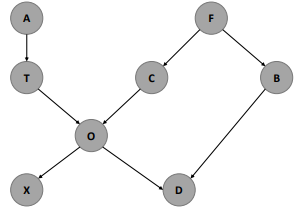
\includegraphics[width=.4\linewidth]{excercise2f}
	  	\caption{Modelo gráfico de diagnóstico de enfermedades de pulmón.}
	  	\label{fig1}
	  \end{figure}
	A una clínica le concierne el diagnóstico de enfermedades de pulmón. Como se puede ver en el modelo de la Figura~\ref{fig1}, una visita a Asia ($A$) hace que la probabilidad de tener tuberculosis ($T$) aumente. Los nodos en la gráfica tienen el siguiente significado:	 
	\begin{figure}[h!]
		\centering
		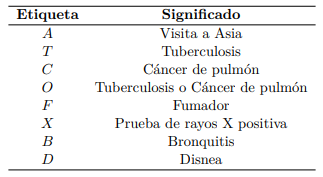
\includegraphics[width=.4\linewidth]{excercise2t}
		\label{table1}
	\end{figure}
Di si las siguientes relaciones de independencia condicional son verdaderas o falsas y explica por qué:
\subsection{$T  \perp\!\!\!\perp F | D$}
\subsection{$C  \perp\!\!\!\perp B | F$}
\subsection{$A  \perp\!\!\!\perp F | C$}
\subsection{$A  \perp\!\!\!\perp F | C,D$}
\section{Ejercicio 3}
Imagina una clínica que ayuda a pacientes con ébola en un área afectada por el virus. La red de la Figura~\ref{fig2} intenta capturar la dinámica por la cual las personas que sufren los síntomas pueden llegar a esta clínica y ver a un especialista. Existe la posibilidad de que alguien con ébola ($E=\text{verdadero}$) muestre síntomas, por ejemplo sangrado ($S=\text{verdadero}$), fiebre ($F=\text{verdadero}$) y visite la clínica ($V=\text{verdadero}$). El sangrado incrementa el riesgo de complicaciones ($C=\text{verdadero}$) y la persona puede ser llevada a ver un doctor especialista ($D=\text{verdadero}$).
\begin{figure}[h!]
	\centering
	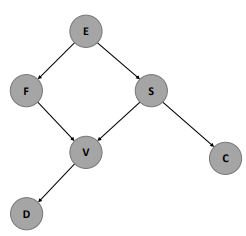
\includegraphics[width=.35\linewidth]{excercise3f}
	\caption{Modelo gráfico de detección de ébola.}
	\label{fig2}
\end{figure}
\pagebreak
\begin{itemize}
	\item $P(E=\text{verdadero})=0.01$
	\item $P(F=\text{verdadero}|E=\text{verdadero})=0.6$
	\item $P(F=\text{verdadero}|E=\text{falso})=0.1$
	\item $P(S=\text{verdadero}|E=\text{verdadero})=0.8$
	\item $P(S=\text{verdadero}|E=\text{falso})=0.05$
	\item $P(V=\text{verdadero}|F=\text{verdadero},S=\text{verdadero})=0.8$
	\item $P(V=\text{verdadero}|F=\text{verdadero},S=\text{falso})=0.5$
	\item $P(V=\text{verdadero}|F=\text{falso},S=\text{verdadero})=0.7$
	\item $P(V=\text{verdadero}|F=\text{falso},S=\text{falso})=0.0$
	\item $P(C=\text{verdadero}|S=\text{verdadero})=0.75$
	\item $P(C=\text{verdadero}|S=\text{falso})=0.1$
	\item $P(D=\text{verdadero}|V=\text{verdadero})=0.6$
	\item $P(D=\text{verdadero}|V=\text{falso})=0.0$
\end{itemize}
Con estas probabilidades y el modelo gráfico de la Figura~\ref{fig2}, realiza lo siguiente:
\subsection{} Escribe la distribución conjunta de la red bayesiana en función de las probabilidades condicionales.
\subsection{} Si un paciente es llevado al doctor ($D=\text{verdadero}$), usando un paquete de software calcula la probabilidad de que no tenga ébola  ($P(E=\text{falso}|D=\text{verdadero})$).
\subsection{} Convierte a la red bayesiana en un modelo gráfico no dirigido (campo aleatorio de Markov) y dibújalo. Captura tantas relaciones de independencia condicional como sea posible.
\subsection{} Debido a una campaña de concientización de la salud, las personas son alentadas a visitar la clínica en caso de que tengan fiebre. Esto incrementa la cantidad de visitas de personas con fiebre sin importar el estado de cualquier otra variable.
\subsubsection{} ¿Qué probabilidades condicionales en la red se modifican debido a este cambio y en qué sentido?
\subsubsection{} Describe cualquier efecto que esto tenga en la proporción de personas con complicaciones que visiten la clínica. Menciona exactamente qué probabilidades condicionales usaste para llegar a tu conclusión.
\subsection{} Asume que alguien que no tiene fiebre va al doctor, ¿qué relación de independencia condicional existe en la distribución que no puede ser descubierta a través del grafo solamente?
 \subsection{Opcional} Calcula $P(V|E=\text{verdadero})$ usando el método de eliminación de variables, describiendo de forma detallada el procedimiento que seguiste (2 puntos extras).
\end{document}  